%% FSE (CS-5187 Term Project) research paper. Requirements from the CFP (https://conf.researchr.org/home/fse-2026, checked 2026-09-30):
%%   * \documentclass[acmsmall,screen]{acmart}; single column
%%   * 12 pages of text and figures + references limit \todo{check}
%%   * double-anonymous: no names, no identifying URLs, third-person
%%     self-citation, no acknowledgments at submission
%%   * "Data Availability" section after the Conclusion (not counted)
%%   * disclose AI tools; fabricated citations = desk reject
%%   * deadline: TODO (see course page) AoE, TODO
%% Used for e.g. FSE, ISSTA, OOPSLA/PACMPL, TOSEM.
\documentclass[acmsmall,screen]{acmart}

%% Shared macros. Keep notation here so the paper cannot drift from itself.
%% Rule: every name, symbol and set used more than once gets a macro here.
\usepackage{amsmath}
\usepackage{booktabs}
\usepackage{xspace}
\usepackage{listings}
\usepackage{xcolor}
\usepackage{array}
\usepackage{pifont}
\usepackage{tikz}
\usetikzlibrary{arrows.meta,positioning,calc,fit,backgrounds}
\DeclareRobustCommand{\circled}[1]{\tikz[baseline=(c.base)]\node[circle,draw,inner sep=0.7pt,font=\tiny\bfseries] (c) {#1};}

% ---- project name (anonymised for review) ----
% Works for any CS-5187 project: a tool, a technique/method, or an empirical
% study. With no tool (e.g. a study), read \tool as "our study" and reword
% "We present \tool" -> "We study ...", "\tool records" -> "our method ...".
\newcommand{\tool}{\textsc{SLDF}\xspace}   % Semantic LLM-Directed Fuzzing: the framework of all four methods

% ---- notation (one macro per symbol; comment says what it means) ----
% \newcommand{\Seen}[1]{\ensuremath{\mathit{Seen}(#1)}} % example: lines the compiler sees

% ---- research questions ----
\newcommand{\rqref}[1]{\textbf{RQ#1}\xspace}

% ---- results: one boxed, numbered claim per observation ----
\newcounter{observation}
\newsavebox{\obsbox}
\newenvironment{observation}
  {\refstepcounter{observation}\par\smallskip\noindent\begin{lrbox}{\obsbox}\begin{minipage}{0.95\linewidth}\textbf{Observation~\theobservation.}~}
  {\end{minipage}\end{lrbox}\fbox{\usebox{\obsbox}}\par\smallskip}

% ---- CS-5187 term-project FOCUS callouts (RED, on purpose) ----
% A red box that marks a part every term-project report MUST address:
%   Research Questions, Motivating Example, Workflow, Related Work,
%   Threats to Validity. The red is a study aid, not paper style -- once
%   you have written the section, DELETE its \focus{...} line (keep the
%   section). A finished report has zero \focus and zero \todo.
\newcommand{\focus}[1]{%
  \par\smallskip\noindent
  {\color{red}\rule{\linewidth}{0.6pt}}\par\nobreak\vspace{1pt}\noindent
  {\color{red}\ding{228}~\textbf{FOCUS --- graded, must address:}~\itshape #1}\par\nobreak\vspace{1pt}
  {\color{red}\rule{\linewidth}{0.6pt}}\par\smallskip}

% ---- editorial (all must be gone before submission; scripts/check.sh counts them) ----
\newcommand{\todo}[1]{\textcolor{red}{[TODO: #1]}}
\newcommand{\num}[1]{\textcolor{blue}{#1}}   % a number not yet measured by the final tool
\newcommand{\cmark}{\ding{51}}
\newcommand{\xmark}{\ding{55}}

\lstset{basicstyle=\ttfamily\footnotesize,columns=fullflexible,
        keepspaces=true,frame=single,framesep=2pt,xleftmargin=4pt,
        numbers=left,numberstyle=\tiny,numbersep=4pt}

% long \texttt words otherwise run into the margin
\setlength{\emergencystretch}{3em}


\setcopyright{none}
\acmConference[FSE (CS-5187 Term Project)]{ACM International Conference on the Foundations of Software Engineering (Format Template)}{2026}{IIT Guwahati}
\acmYear{2026}
\citestyle{acmauthoryear}

\begin{document}

\title[LLM-Directed Fuzzing of DuckDB]{Semantic LLM-Directed Fuzzing of DuckDB: Four Methods, One Judge, and 16 Upstream Bugs}
%% Title pattern: "Short Hook: Plain Description of What and For Whom".
%% Alternative titles (keep 2-3 here until submission):
%%   "..."

\author{Prabhnoor}
\affiliation{\institution{IIT Guwahati}\city{Guwahati}\country{India}}
\author{Niket Garg}
\affiliation{\institution{IIT Guwahati}\city{Guwahati}\country{India}}
\author{Janhvi Mittal}
\affiliation{\institution{IIT Guwahati}\city{Guwahati}\country{India}}

\begin{abstract}
A query optimizer that rewrites a query wrongly returns a wrong answer without any error, so users have no reason to
doubt it. Random SQL fuzzers rarely reach the narrow conditions under which a single rewrite rule fires, and a bug
found in a released version is often already fixed in the development branch. We present \tool, a framework of four
fuzzing methods for the DuckDB database that run side by side and share one execution judge, one oracle layer and one
triage pipeline: (A) classic generic fuzzing as a baseline, (B) fuzzers aimed at features new in DuckDB~2.0, (C) test
generators written by a large language model (LLM) and guided by new-code hints and fix dossiers, and (D) a
rule-targeted loop. Method D mines a \emph{rule card} for each optimizer rule from its source code and fix history,
asks the LLM for a bug hypothesis and a generator program, and accepts the generator only if executing it shows that
the target rule fired. With these methods we filed 16 issues on DuckDB~2.0.0: 8 silent wrong results, 5 internal
errors and 3 spurious errors. Maintainers have fixed 4 of them, 9 more have open fix pull requests (one of them ours),
and Method D alone found 12. One unattended run of Method D spent 40 LLM calls on 13 targets and produced 9 candidates
that became 6 issues. Generic fuzzing with 70{,}980 SQLsmith queries found no new bug.

\end{abstract}

%% CCS concepts: pick the ones that fit YOUR project at https://dl.acm.org/ccs
%% (500 = main, 300 = secondary). This template fits any software-engineering
%% topic -- static analysis, dynamic analysis/testing, empirical studies,
%% program repair, tools, human factors, etc. -- so replace the placeholder
%% below with the concept for your own work. A few common top-level ids:
%%   Software and its engineering~Software testing and debugging
%%   Software and its engineering~Automated static analysis
%%   Software and its engineering~Dynamic analysis
%%   Software and its engineering~Software creation and management
%%   General and reference~Empirical studies
\begin{CCSXML}
<ccs2012>
  <concept>
    <concept_id>10011007.10011074.10011099.10011102.10011103</concept_id>
    <concept_desc>Software and its engineering~Software testing and debugging</concept_desc>
    <concept_significance>500</concept_significance>
  </concept>
</ccs2012>
\end{CCSXML}
\ccsdesc[500]{Software and its engineering~Software testing and debugging}

\keywords{fuzzing, database testing, query optimizer, differential testing, large language models, DuckDB}

\maketitle

\section{Introduction}
\label{sec:intro}

Suppose a data analyst filters a table of measurements with \texttt{WHERE -d > 'nan'::DOUBLE}. The database plans the
query, its optimizer rewrites the predicate into a cheaper form, and the analyst receives rows. Nothing fails and no
warning appears. If the rewrite was wrong, the analyst has no way to notice. Database testing tools such as
SQLancer~\cite{rigger2020tlp,rigger2020norec} and grammar-based fuzzers such as SQLsmith~\cite{sqlsmith} and
Squirrel~\cite{zhong2020squirrel} were built for this class of \emph{logic bug}. They generate many queries and compare
each answer with an answer that should be equal.

These tools work best on code that random queries reach often. An optimizer, however, is a long list of small rewrite
rules, and each rule fires only under narrow conditions: a constant of a specific type, a cast next to a comparison, a
join key of a list type. A rule that fires on one query in ten thousand is tested rarely, and its edge cases (type
limits, signed zero, NaN) more rarely still. A second problem is timing. Projects such as
DuckDB~\cite{raasveldt2019duckdb} are fuzzed continuously by their developers and by other researchers, so a bug found
in a release is often already fixed on the development branch. In our first month, every real bug our tools found in
DuckDB~1.5.6 had already been reported or fixed upstream (Section~\ref{sec:eval-methods}).

We focus on a third problem that starts where these tools stop: \emph{directing} the search at one optimizer rule at a
time, and proving that the generated tests actually exercise that rule. Large language models (LLMs) can read source
code and write programs, which makes directed generation possible~\cite{yang2024whitefox,xia2024fuzz4all}. But an LLM
also reports success it did not achieve. In an early run of our pipeline, 10 of 11 generators that an LLM agent wrote
and described as thorough produced exactly 8 queries per case and 5 to 12 distinct plans
(Section~\ref{sec:eval-judge}).

\paragraph{A real example.} Figure~\ref{fig:motivating} shows issue \#28052, which one of our LLM-written generators
found in DuckDB~2.0.0. DuckDB orders NaN above every other value, so \texttt{-d > NaN} is false for every row. The rule
\texttt{MoveUnaryMinusRule} rewrites \texttt{-x > c} into \texttt{x < -c}. Its guard handles a NaN \emph{column value}
but not a NaN \emph{constant}, so the query returns all 4 rows instead of none. With the expression rewriter switched
off, DuckDB returns the correct empty result, and DuckDB~1.5.6 was also correct. The maintainers merged a fix one day
after we filed (PR \#28071). This is not a single case: 8 of the 16 issues we filed are silent wrong results
(Table~\ref{tab:issues}).

\begin{figure}[t]
\begin{lstlisting}[basicstyle=\ttfamily\footnotesize,frame=single,columns=fullflexible]
CREATE TABLE f(d DOUBLE);
INSERT INTO f VALUES (1.5), (-2.5), ('nan'), ('inf');
SELECT d FROM f WHERE -d > 'nan'::DOUBLE ORDER BY d;
  -- DuckDB 2.0.0:  -2.5, 1.5, inf, nan     (4 rows, wrong)
  -- expected:      no rows                  (NaN is the largest value)
SET disabled_optimizers = 'expression_rewriter';
SELECT d FROM f WHERE -d > 'nan'::DOUBLE ORDER BY d;   -- no rows (correct)
\end{lstlisting}
\caption{Issue \#28052, found by an LLM-written generator. One rewrite rule turns an always-false predicate into an
always-true one. No error is raised; only a second run with the rule switched off shows the difference.}
\label{fig:motivating}
\end{figure}

Closest to our work, WhiteFox~\cite{yang2024whitefox} lets an LLM read compiler optimization code and write tests for
it, and directed greybox fuzzing~\cite{bohme2017aflgo} steers inputs toward chosen code locations. However, WhiteFox
targets compilers and trusts the LLM's description of what triggers an optimization, and directed greybox fuzzers need
distances over a control-flow graph, which is costly to compute for a large C++ database. Neither checks with the
database itself that a generated SQL test fired the intended rewrite.

\paragraph{Our approach.} We present \tool (Semantic LLM-Directed Fuzzing), a framework of four methods that run side
by side on the same infrastructure (Section~\ref{sec:approach}):
\begin{enumerate}
  \item \textbf{Method A, classic fuzzing}, as a baseline and safety net: SQLsmith on a sanitizer build, differential
        sweeps of DuckDB's own tests, and replay of past bug reports (Section~\ref{sec:method-a}).
  \item \textbf{Method B, feature-targeted fuzzers} for features that are new in DuckDB~2.0, such as triggers
        (Section~\ref{sec:method-b}).
  \item \textbf{Method C, new-code hints and LLM-written generators}: the LLM receives hints about code that is new or
        never executed, feature cards and fix dossiers, and writes a generator program (Section~\ref{sec:method-c}).
  \item \textbf{Method D, the rule-targeted loop}: a \emph{rule card} per optimizer rule, mined from its source and fix
        history, a hypothesis-first LLM generator, and an \emph{engine judge} that accepts the generator only if the rule
        fires on its queries (Section~\ref{sec:method-d}).
\end{enumerate}
All four methods feed one oracle layer and one triage pipeline. A person reads every surviving candidate before
anything is filed.

\paragraph{Results.} Over five weeks we filed 16 issues on DuckDB~2.0.0. Maintainers fixed 4 (\#27759, \#27850,
\#28052, \#28562), 9 more have open fix pull requests, and one of those (\#28547) is ours. Method D found 12 of the 16.
One unattended run of Method D spent 40 LLM calls on 13 targets, ran 32 generator rounds and turned 597 raw differences
into 9 triaged candidates and 6 issues (Table~\ref{tab:hunt1}). The main lesson is that the LLM is useful only when the
engine checks its work, and that the check must not be the only gate: four generators that found bugs failed our own
diversity floor, so we triage the hits of every generator but count only judged generators as test coverage.

\paragraph{Contributions.}
\begin{itemize}
  \item A framework of four complementary fuzzing methods for a database optimizer that share one judge, one oracle
        layer and one triage pipeline (Section~\ref{sec:approach}).
  \item Rule cards: per-rule targets mined from source code and fix history, including the early exits under which a
        rewrite fires and the places where it builds values (Section~\ref{sec:method-d}).
  \item An engine judge that measures rule-level reach and rejects generators that only claim it, checked by positive
        and negative controls (Sections~\ref{sec:judge} and~\ref{sec:eval-judge}).
  \item 16 upstream issues on DuckDB with minimal reproducers, 4 of them fixed, and one fix pull request
        (Section~\ref{sec:evaluation}). All code and data are public (Section~\ref{sec:data}).
\end{itemize}

\section{Background}
\label{sec:background}

\paragraph{DuckDB and its optimizer.} DuckDB~\cite{raasveldt2019duckdb} is an embedded analytical database written in
C++. A query passes through a parser, a binder, an optimizer and a vectorized executor. In DuckDB~2.0.0 the optimizer applies
a fixed sequence of 46 passes (for example filter pushdown, join ordering, removal of unused columns, top-N window
elimination). One pass, the \emph{expression rewriter}, applies small \emph{rules} (29 source files in
\texttt{src/optimizer/rule}) to every expression, for example
moving constants across a comparison or simplifying a \texttt{date\_trunc}. The setting
\texttt{disabled\_optimizers} switches off a named pass; a rule can only be switched off together with its whole pass.
We call this a \emph{switch}. DuckDB~2.0.0 was released during our project; we tested that release and checked every
candidate on the newest development build (\emph{main}).

\paragraph{Logic bugs and oracles.} A \emph{logic bug} makes the database return a wrong result without an error. To
detect one, a fuzzer needs an \emph{oracle}: a second computation whose result must be equal. Differential testing
compares two systems or two configurations of one system. Ternary logic partitioning (TLP)~\cite{rigger2020tlp} splits a
query by a predicate into three parts that must add up to the original. NoREC~\cite{rigger2020norec} compares an
optimized query with a form the optimizer cannot rewrite. Our main oracle is differential: the same query with a switch on
and off. An \emph{internal error} is DuckDB's own assertion that an impossible state was reached; a \emph{spurious error}
is an error raised for a valid query that should succeed.

\paragraph{Reach.} A test for a rule is useful only if the rule fires on it. We say a query \emph{reaches} a target
when its plan changes when the target's switch is turned off (\emph{expression-level reach}), and, more strictly, when a
call that only the target rule removes disappears from the plan (\emph{rule-level reach}). The fraction of valid queries
that reach the target is the \emph{reach rate}.

\paragraph{Terms used later.} A \emph{generator} is a short Python program that returns test cases (a setup script and
queries); an LLM writes it, our harness runs it. A \emph{hit} is a raw difference between configurations. A
\emph{candidate} is a hit that survived automatic triage. An \emph{issue} is a candidate a person checked and filed upstream.


\section{Approach}
\label{sec:approach}

%% Figure: overview of SLDF. Four methods (top) feed one shared core (bottom).
\begin{figure}[t]
\centering
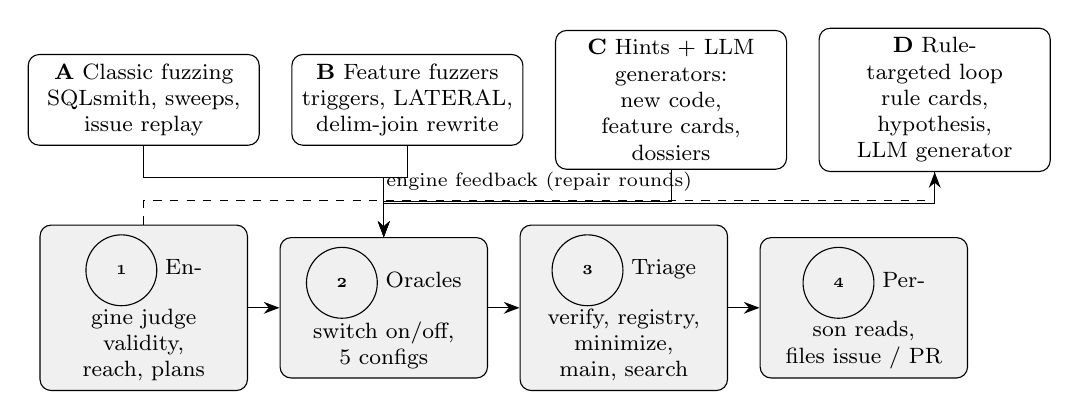
\begin{tikzpicture}[font=\footnotesize, node distance=4mm,
  m/.style={draw, rounded corners, align=center, minimum height=11mm, text width=27mm},
  c/.style={draw, rounded corners, align=center, minimum height=9mm, text width=24mm, fill=black!6},
  >={Stealth[length=2mm]}]
\node[m] (a) {\textbf{A} Classic fuzzing\\SQLsmith, sweeps,\\issue replay};
\node[m, right=of a] (b) {\textbf{B} Feature fuzzers\\triggers, LATERAL,\\delim-join rewrite};
\node[m, right=of b] (cc) {\textbf{C} Hints + LLM\\generators: new code,\\feature cards, dossiers};
\node[m, right=of cc] (d) {\textbf{D} Rule-targeted loop\\rule cards, hypothesis,\\LLM generator};
\node[c, below=10mm of a] (j) {\circled{1} Engine judge\\validity, reach, plans};
\node[c, right=of j] (o) {\circled{2} Oracles\\switch on/off, 5 configs};
\node[c, right=of o] (t) {\circled{3} Triage\\verify, registry,\\minimize, main, search};
\node[c, right=of t] (h) {\circled{4} Person reads,\\files issue / PR};
\draw[->] (j) -- (o); \draw[->] (o) -- (t); \draw[->] (t) -- (h);
\foreach \x in {a,b,cc,d} { \draw[->] (\x.south) -- ++(0,-4mm) -| (o.north); }
\draw[->, dashed] (j.north) -- ++(0,3mm) -| node[pos=0.25, above, font=\scriptsize]{engine feedback (repair rounds)} (d.south);
\end{tikzpicture}
\caption{\tool: four fuzzing methods run side by side and share one core. Generators written by an LLM (Methods C and D)
pass the engine judge \circled{1} first, which also returns measured feedback for the next round of Method D. Every hit
goes through the same oracles and triage, and a person decides what is filed.}
\label{fig:overview}
\end{figure}


\tool consists of four fuzzing methods and one shared core (Figure~\ref{fig:overview}). The methods differ in
\emph{where} they look and \emph{who} writes the tests. The core decides \emph{whether} a test is meaningful and
\emph{whether} a difference is a bug. We ran the methods side by side, not one after the other: each covers a blind
spot of the others, and a new method can be added without changing the core. We first describe the core
(Section~\ref{sec:core}), then the four methods (Sections~\ref{sec:method-a}--\ref{sec:method-d}).

\subsection{The Shared Core}
\label{sec:core}

\paragraph{\circled{1} The engine judge.}
\label{sec:judge}
An LLM-written generator is run on DuckDB, and its quality is measured by the database, not reported by the LLM. For a
generator with target switch $s$, the judge runs every query once with $s$ on and once with $s$ off and records:
the \emph{valid rate} (queries DuckDB accepts); the \emph{reach rate} (Section~\ref{sec:background}); the number of
distinct physical operator trees, read from \texttt{EXPLAIN (FORMAT JSON)}; and the number of distinct query
\emph{skeletons}, that is, queries with identifiers and literals removed. A generator is rejected as \emph{low
diversity} if any hard flag holds: fewer than $\max(30, 0.02 n)$ skeletons for $n$ valid queries; fewer than
$\max(15, 0.03 c)$ operator trees for $c$ cases; a reach rate below 30\%; fewer than half of the valid queries taking
part in the result comparison; or a rule target without a marker function. For a rule target, reach must be
\emph{rule-level}: the rule card names a function call that only this rule removes, and the call must disappear from
the plan. A generator that names the rule but never gives it a bare column passes expression-level reach but fails
rule-level reach (Section~\ref{sec:eval-judge}).

\paragraph{\circled{2} Oracles.} Each query runs under five configurations: the default; the target switch off;
\texttt{delim\_join\_as\_cte=false} (a rewrite new in 2.0); one thread; and \texttt{PRAGMA enable\_verification}, which
makes DuckDB re-run each query in several internal ways. A \emph{config difference} is a result that differs from the
default. An \emph{error difference} is an error raised in one configuration only; if only the optimized run fails, the
optimizer turned a valid query into a failing one. Results are compared as multisets after normalizing values close to
zero, and queries whose order is undefined are excluded. The generator contract requires unique sort keys, because ties
under \texttt{ORDER BY} or \texttt{row\_number()} are the first source of false alarms.

\paragraph{\circled{3} Triage.} Every hit, from any method, passes five automatic steps: (1) \emph{verify}: replay the
script alone and in a fresh process, and drop it if the difference disappears; (2) \emph{registry}: compare the
signature with our registry of known issues, which labels it a rediscovery, a sibling or new; (3) \emph{minimize}:
greedy delta reduction over statements and then over rows of \texttt{VALUES} lists, keeping the same verdict;
(4) \emph{main}: run the minimized script on the newest development build and drop it if it is fixed there; (5)
\emph{search}: query GitHub for issues and pull requests with the same function, rule or error text. Hits where the
optimizer only hides an error (the unoptimized run fails, the optimized one succeeds) are labelled low priority,
because DuckDB accepts this behaviour.

\paragraph{\circled{4} The person.} Triage writes a list of candidates with minimized reproducers. A team member reads
each one, decides which side is right by reading the rule's code, and writes the issue. Nothing is filed
automatically. We grouped siblings with one root cause into one issue.

\subsection{Method A: Classic Fuzzing}
\label{sec:method-a}

Method A is generic, undirected fuzzing. It runs SQLsmith~\cite{sqlsmith} against an AddressSanitizer and
UndefinedBehaviorSanitizer build of DuckDB, sweeps the 2{,}560 SQL scripts we extracted from DuckDB's own test suite
under the five configurations, mutates them (boundary values, join swaps, nesting), and replays reproducers mined from
closed upstream issues. It needs no LLM and no target. We keep it running as a baseline and as a safety net for memory
errors, which the other methods do not look for.

\subsection{Method B: Feature-Targeted Fuzzers}
\label{sec:method-b}

Method B aims at features that are new in DuckDB~2.0 and rarely appear in the upstream issue stream. Each fuzzer is
hand-written for one feature and has its own oracle. The trigger fuzzer builds random trigger definitions and
data-changing statement sequences and checks three things: the final table equals an emulation of the triggers in
plain SQL, the result survives a restart, and no internal error occurs. Further fuzzers cover window functions with
mixed types, join equivalences (a \texttt{NATURAL JOIN} against \texttt{INTERSECT ALL}), bottom-up query
construction, and the new \texttt{delim\_join\_as\_cte} rewrite, which they compare on and off.

\subsection{Method C: New-Code Hints and LLM-Written Generators}
\label{sec:method-c}

Method C points an LLM at code that is new or never executed. Its inputs are: (1) \emph{static hints}: 24{,}816
branches, boundary constants and risky operations extracted from DuckDB's C++ with tree-sitter, of which 80.9\% are
never executed by the seed corpus of 2{,}560 test scripts; (2) \emph{new-code hints}: the code that changed between
DuckDB~1.5 and 2.0; (3) \emph{feature cards}: a short plain-language description of a new feature and its switches; and
(4) \emph{fix dossiers}: the diff and test of a recent fix, so that the LLM can look for a variant the fix missed. The
LLM writes a generator under a fixed contract (deterministic output, unique sort keys, a declared target switch), and
the engine judge measures it. A one-command, resumable 12-hour run (\texttt{targeted\_run}) drives the loop and ends
with an audit that recomputes every quality verdict from stored counts. We ran Method C with three models: a local
1.5B-parameter model in a pilot, Gemini~2.5~Pro (run by a team member), and Claude in an interactive authoring arm.

\subsection{Method D: The Rule-Targeted Loop}
\label{sec:method-d}

Method D directs the search at one optimizer rule at a time. It has four steps.

\paragraph{Step 1: Rule cards.} For every rule file and optimizer pass, a script builds a \emph{rule card} from the
source and the git history: (a) the commits since March 2026 that touched the file, the fixes among them, and the tests these fixes added (a fix usually covers only the reported case, and the next bug is often in the case next to it); (b)
every early exit in the rule's \texttt{Apply} or \texttt{CanOptimize} function, that is, the exact conditions under
which the rewrite fires; (c) every place where the rule builds or converts a value (bounds, folded constants, casts);
and (d) its marker function and its switch. Cards are ranked by
$\mathit{score} = 2\min(\mathit{fixes},6) + \min(\mathit{commits},15) + 3\min(\mathit{sites},10) + 15[\mathit{rule}] +
5[\mathit{marker}]$, which favours expression rules that build values and were fixed recently. For DuckDB~2.0.0 the
script builds 49 cards.

\paragraph{Step 2: Hypothesis-first generation.} The LLM receives one card and reads the real DuckDB source with
read-only tools (Read, Grep, Glob). Its working directory is an empty folder, so it never sees our issue drafts,
our controls or earlier generators. It must state a bug hypothesis and the preconditions under which the rule fires
(\texttt{META["hypothesis"]}, \texttt{META["preconditions"]}); the judge rejects a rule-targeted generator without
them. The prompt gives three recipes that worked for us: take constants from the generated rows (so that \texttt{=}
can match) and from a list of 275 literals at the limits of 30 types (type maxima, $-0.0$, infinity, extreme dates);
place the target pattern in varied contexts (\texttt{WHERE}, \texttt{SELECT}, \texttt{CASE}, \texttt{FILTER},
\texttt{JOIN ON}, subqueries); and keep queries deterministic.

\paragraph{Step 3: Judge and repair.} The judge runs the generator on 300 cases. Its measured feedback (valid rate,
reach rate, the most common errors, queries that reached the target and queries that did not) becomes the prompt of the
next round. Round 1 of a target uses a larger model (Claude Opus), and repair rounds use a smaller one (Claude Sonnet).
A target retires after three rounds. A generator that the judge accepts and that produced hits is re-run at scale
(1{,}500 cases).

\paragraph{Step 4: Triage of every hit.} All hits go to the shared triage, including hits of generators the judge
rejected. We made this choice after we saw that narrow, deep generators find bugs but have few plan shapes
(Section~\ref{sec:eval-judge}). The judge therefore decides what counts as tested coverage, and triage decides what
counts as a bug.

\paragraph{Running unattended.} The loop keeps a ledger of targets, rounds and candidates, so a stopped run resumes
where it stopped. A failed LLM call is not counted, the loop backs off, and after four failures in a row (for example a
usage limit) it stops cleanly without retiring targets. A supervisor restarts it after a crash. Before every unit it
checks free memory and pauses below 1.5\,GB, and it keeps the laptop awake while it runs.

\paragraph{Why not let the LLM write queries directly?} A generator is a program: one LLM call yields hundreds of
different queries, and the judge can measure the program instead of trusting a handful of examples. In our runs one call
produced 300 to 1{,}500 test cases.

\section{Implementation}
\label{sec:implementation}

\tool is about 11{,}000 lines of Python in \texttt{src/harness}, plus a C++ driver that runs SQL in-process on the
sanitizer build. The main parts are: \texttt{gen\_runner.py} (the engine judge and the five-configuration oracle),
\texttt{verify\_finding.py} and \texttt{gen\_triage.py} (triage), \texttt{known\_issues.json} (the registry),
\texttt{rule\_targets.py} (rule cards), \texttt{edge\_values.py} (the 275 type-limit literals),
\texttt{hunt\_loop.py} with \texttt{hunt\_start.sh} (the unattended loop of Method D), \texttt{targeted\_run.py}
(Method C), and the fuzzers of Methods A and B. The LLM in Method D is Claude Code in headless mode
(\texttt{claude -p}) with only the Read, Grep and Glob tools allowed.
\texttt{controls/check\_controls.py} runs the positive and negative controls after every change to the judge or the
triage. All runs pin the time zone to UTC, because DuckDB's default time zone follows the process environment.

\section{Evaluation}
\label{sec:evaluation}

We answer four research questions.
\begin{description}
  \item[\rqref{1} Effectiveness.] How many previously unknown bugs does \tool find in DuckDB~2.0.0, of which kinds, and
        how do maintainers respond?
  \item[\rqref{2} Methods.] What does each of the four methods contribute, and at what cost?
  \item[\rqref{3} Judge.] Does the engine judge separate generators that exercise their target from generators that
        only claim to?
  \item[\rqref{4} Loop.] How efficient is the unattended rule-targeted loop, from LLM calls to filed issues?
\end{description}

\paragraph{Setup.} All runs of Methods A, B and D and the Claude arm of Method C used one laptop: an Intel Core
i3-1315U (8 hardware threads), 7.4\,GB of RAM under WSL2 (Linux 6.18), Python~3.14.4 and the released DuckDB~2.0.0
(source tag \texttt{v2.0.0}); Method A on DuckDB~1.5.6 and~2.0.0 used our own sanitizer builds. The LLM of Method D was
Claude Code~2.1.323 with Claude Opus for the first round of each target and Claude Sonnet for repair rounds, on a
personal subscription. Round~2 of Method C ran on a team member's machine with Gemini~2.5~Pro. Workers ran one at a
time with a DuckDB memory limit, because larger settings froze the machine. Every number in this section is produced
by \texttt{paper/scripts/collect\_data.py} and \texttt{collect\_extra.py} from run logs and from the GitHub state of our
issues on 13~November~2026; the outputs are in \texttt{paper/data}.

\subsection{RQ1: Bugs Found}
\label{sec:eval-bugs}

%% generated by paper/scripts/collect_data.py from data/issues.csv
\begin{table*}[t]
\caption{All 16 issues we filed on DuckDB. \emph{Method}: the method of Section~\ref{sec:approach} that found it. \emph{Kind}: wrong result (silent), internal error (an assertion or INTERNAL Error, in two cases also invalidating the database), or spurious error (a valid query fails). \emph{Status} on 2026-11-13; fix PRs are by maintainers or other contributors, except \#28547 (ours).}
\label{tab:issues}
\footnotesize\centering
\begin{tabular}{llllp{4.1cm}}
\toprule
Issue & Method & Kind & What goes wrong & Status \\
\midrule
\#27759 & B & internal error & FOR EACH ROW trigger into a table with a BEFORE INSERT trigger & fixed (PR \#28698) \\
\#27850 & C & internal error & identical EXISTS blocks under UNION ALL (delim\_join\_as\_cte=false) & fixed (PR \#28144) \\
\#27904 & C & internal error & CROSS JOIN LATERAL with a nested LATERAL count(*) & open, fix PR \#27975 \\
\#28052 & C & wrong result & negated DOUBLE compared with a NaN constant & fixed (PR \#28071) \\
\#28527 & D (session) & wrong result & date\_trunc with a sub-day part on a DATE column & open, fix PR \#28528 \\
\#28531 & D (session) & spurious error & CAST(timestamp AS DATE) = date at the TIMESTAMP range limits & open, fix PR \#28547 \\
\#28532 & D (session) & internal error & TIMESTAMP\_MS to TIMESTAMP\_S cast at range end invalidates the database & open, fix PR \#28539 \\
\#28534 & D (session) & spurious error & date\_trunc comparison near the end of the TIMESTAMP range & open \\
\#28535 & D (session) & internal error & UBIGINT constant above BIGINT max in x + c1 = c2 & open, fix PR \#28540 \\
\#28536 & D (loop) & wrong result & regex empty group (?:) at the pattern edge treated as an anchor & open, fix PR \#28538 \\
\#28541 & D (loop) & wrong result & UHUGEINT constant above HUGEINT max wraps in x + c1 = c2 & open, fix PR \#28549 \\
\#28542 & D (loop) & wrong result & TRY\_CAST(date AS TIMESTAMP) comparison returns false instead of NULL & open \\
\#28559 & D (loop) & wrong result & top-N window elimination returns the other join side for 0.0 / -0.0 & open, fix PR \#28666, \#28728 \\
\#28562 & D (loop) & wrong result & contains(list, '') returns true for lists without an empty string & fixed (PR \#28563) \\
\#28565 & D (loop) & spurious error & CASE guard around a STRUCT field cast ignored & open, reproduced \\
\#28566 & D (loop) & wrong result & both sides of a DOUBLE[] join key merged for [0.0] and [-0.0] & open, fix PR \#28728 \\
\bottomrule
\end{tabular}
\end{table*}


Table~\ref{tab:issues} lists the 16 issues we filed between 23~October and 9~November~2026; a team member filed one
(\#27904) and another team member filed the rest. Each issue has a minimized reproducer, the affected versions, and the
result with the responsible switch turned off. By kind, 8 are silent wrong results, 5 are internal errors, and 3 are
spurious errors on valid queries. Two of the internal errors are severe: \#28532 invalidates the whole database, so
every later query in the session fails, and \#27759 aborts a trigger cascade.

Maintainers have fixed 4 issues: \#28052 (PR \#28071), \#27850 (PR \#28144), \#28562 (PR \#28563) and \#27759
(PR \#28698, which also fixes a related wrong result; DuckDB's lead developer closed the issue). For 9
more issues a fix pull request is open; 8 of them were written by maintainers or other contributors after reading our
report, and one (\#28547 for \#28531) is ours. DuckDB's bot labelled 11 of the 16 issues as \emph{reproduced}. None was
closed as a duplicate or as expected behaviour.

The bugs cluster in one family: constants at the limits of their type inside optimizer rewrites. The rewrite builds a
new value (a bound, a moved constant, a cast) and that value overflows, wraps or loses a NaN or a sign. In \#28541, a UHUGEINT constant above the HUGEINT maximum silently wraps when it is moved across \texttt{=}. In \#28534, a \texttt{date\_trunc} bound lies one step past the last valid timestamp. In \#28559 and \#28566, the signed zero makes \texttt{[0.0] = [-0.0]} true although the two values print differently.

\begin{observation}
\tool found 16 previously unknown bugs in DuckDB~2.0.0, half of them silent wrong results. Maintainers fixed 4 within three weeks and fix pull requests exist for 9 more; none was rejected.
\end{observation}

\subsection{RQ2: What Each Method Contributes}
\label{sec:eval-methods}

\begin{table}[t]
\caption{What each method ran and what it found. \emph{Work}: tests executed or LLM calls spent. \emph{New}: issues
filed that were previously unknown. Method A ran first on DuckDB~1.5.6 and later on~2.0.0; all its real findings were
already known upstream.}
\label{tab:methods}
\footnotesize\centering
\begin{tabular}{lp{4.4cm}p{4.6cm}rr}
\toprule
Method & Input and LLM & Work & New & Fixed \\
\midrule
A classic & none & 70{,}980 SQLsmith queries (92.3\% valid); 11{,}235 differential queries; 14{,}000 sanitizer runs & 0 & 0 \\
B features & hand-written fuzzers for new 2.0 features & trigger, window, join, bottom-up and delim-join fuzzers & 1 & 1 \\
C hints + LLM & static and new-code hints, feature cards, dossiers; 1.5B local model, Gemini~2.5~Pro, Claude &
  Gemini Round~2: 12 generators, 36{,}600 cases, 122{,}590 valid queries; Claude arm & 3 & 2 \\
D rule loop & rule cards; Claude Opus and Sonnet & interactive session; loop runs \texttt{smoke1} (2 calls) and
  \texttt{hunt1} (40 calls) & 12 & 1 \\
\midrule
Total & & & 16 & 4 \\
\bottomrule
\end{tabular}
\end{table}

Table~\ref{tab:methods} compares the methods. \textbf{Method A} found real failures but no new bug. A differential
sweep of 11{,}235 queries over DuckDB's own tests on DuckDB~1.5.6 surfaced two crashes, both already reported and fixed
upstream; a sanitizer hunt over 14{,}000 runs produced 109 hits with 22 distinct signatures, all of them known bugs or
expected behaviour; and a 45-minute SQLsmith campaign of 70{,}980 queries on the 2.0.0 sanitizer build produced 46 raw
anomalies and no new bug. This is the gap that motivated the other methods: generic fuzzing re-finds what upstream's
own fuzzers already find.

\textbf{Method B} found our first new bug: the trigger fuzzer found \#27759, an internal error when a
\texttt{FOR EACH ROW} trigger inserts into a table that has a \texttt{BEFORE INSERT} trigger. Triggers were new in
DuckDB~2.0 and rarely appeared in upstream reports.

\textbf{Method C} found three bugs (\#27850, \#27904, \#28052), two of them now fixed. Its results depend strongly on
the model. In the pilot with a local 1.5B-parameter model, 72 of 126 guided queries were valid (57\%) and none of 10
targeted code regions was reached. Gemini~2.5~Pro in Round~2 wrote 12 generators that passed the audit and ran
122{,}590 valid queries without a new bug; its four candidates were two sanitizer-only failures already fixed upstream
and two that did not reproduce. The same round shows the cost of directing: the directed generators covered 17.89\% of
DuckDB's 160{,}389 instrumented lines, against 38.64\% for the baseline corpus, because each generator stays close to
one target.

\textbf{Method D} found 12 of the 16 bugs: 5 in an interactive session in which Claude read the optimizer source and its fix history with a person in the loop, and 7 in the unattended loop. Rule cards automate what this session did by hand. These 7 came from 42 LLM calls (Section~\ref{sec:eval-loop}).

\begin{observation}
The methods are complementary. Generic fuzzing found no new bug, a feature fuzzer found the first one, and directing an
LLM at single rules found 12 of 16. A larger model and a narrower target mattered more than more tests: Method C ran
more than 120{,}000 queries in one round without a new bug, and Method D found 6 bugs with 40 calls.
\end{observation}

\subsection{RQ3: Does the Engine Judge Work?}
\label{sec:eval-judge}

\begin{table}[t]
\caption{Controls of the judge and the triage. A control must reach its expected verdict after every change to them.
\emph{Rule}/\emph{Expr.}: rule-level and expression-level reach rate. \emph{Re-found}: the issue that triage classified the
control's hits as a rediscovery of.}
\label{tab:controls}
\footnotesize\centering
\begin{tabular}{llrrrl}
\toprule
Control & Judge verdict & Rule & Expr. & Hits & Re-found \\
\midrule
cheat (names rule, never fires it) & rejected & 0.00 & 0.23 & 0 & -- \\
positive (\texttt{date\_trunc}) & accepted & 0.33 & 0.55 & 8 & \#28527 \\
session generator, arithmetic & rejected (diversity) & 0.59 & 0.59 & 8 & \#28535 \\
session generator, cast comparison & rejected (diversity) & 0.11 & 0.40 & 12 & \#28532 \\
session generator, \texttt{date\_trunc} edges & rejected (diversity) & 0.22 & 0.56 & 6 & \#28534 \\
session generator, timestamp cast & rejected (diversity) & 0.35 & 0.58 & 2 & \#28531 \\
\bottomrule
\end{tabular}
\end{table}

The judge exists because an LLM reports progress it did not make. In the first unattended Method~C run, 10 of 11
generators written by an LLM agent produced exactly 8 queries per case and 5 to 12 distinct plans, and the run's only
reported bug was our own \#27759 again. Our first judge counted SQL keywords instead of operators, which a red-team
review showed could be satisfied without testing anything; we rebuilt it on operator trees from
\texttt{EXPLAIN (FORMAT JSON)}.

Table~\ref{tab:controls} shows the controls we run after every change. The negative control names the target rule but
never gives it a bare column, so constant folding removes the call before the rule sees it. Its expression-level reach
is 0.23, but its rule-level reach is 0.00, and the judge rejects it. The positive control is accepted and its hits are
classified as rediscoveries of \#28527. The four session generators that found \#28531, \#28532, \#28534 and \#28535
still re-find exactly their own bug, so the triage and the registry work end to end.

The same table also shows a limit of the judge. All four session generators fail the diversity floor: they are narrow
and deep, with few query skeletons, yet each found a real bug. For this reason Method D triages the hits of every
generator. In \texttt{hunt1}, the judge accepted 23 of 32 rounds, and all 9 candidates came from accepted rounds; the rejected rounds produced 128 raw hits and no candidate.

\begin{observation}
Measured rule-level reach rejects a generator that only names its target, and controls that re-find our own bugs show
the pipeline still works after every change. The diversity floor is a measure of coverage, not of bug-finding power:
narrow generators can find bugs, so their hits must still be triaged.
\end{observation}

\subsection{RQ4: The Unattended Loop}
\label{sec:eval-loop}

%% generated by paper/scripts/collect_data.py from data/hunt_units.csv and the hunt1 ledger
\begin{table}[t]
\caption{The automated loop (Method D, run \texttt{hunt1}): most targets give nothing, a few give bugs. \emph{Units}: generator rounds run. \emph{OK}: rounds the engine judge accepted. \emph{Reach}: best fraction of valid queries whose plan changes when the target is switched off. \emph{Hits}: raw differences before triage. \emph{Cand.}: hits that survived triage. \emph{Issues}: filed upstream.}
\label{tab:hunt1}
\footnotesize\centering
\begin{tabular}{lrrrrrl}
\toprule
Target & Units & OK & Reach & Hits & Cand. & Issues \\
\midrule
\texttt{remove\_unused\_columns} & 4 & 4 & 1.00 & 95 & 2 & 28565, 28566 \\
\texttt{date\_trunc\_simplification} & 2 & 1 & 0.61 & 0 & 0 & -- \\
\texttt{move\_constants} & 2 & 2 & 0.98 & 98 & 1 & 28541 \\
\texttt{comparison\_simplification} & 2 & 1 & 0.31 & 189 & 1 & 28542 \\
\texttt{monotone\_preimage} & 3 & 3 & 0.80 & 10 & 0 & -- \\
\texttt{timestamp\_comparison} & 3 & 3 & 0.77 & 3 & 0 & -- \\
\texttt{string\_prefix} & 3 & 2 & 0.64 & 1 & 0 & -- \\
\texttt{topn\_window\_elimination} & 3 & 3 & 0.97 & 108 & 4 & 28559 \\
\texttt{in\_clause\_simplification\_rule} & 3 & 1 & 0.37 & 60 & 0 & -- \\
\texttt{compressed\_materialization} & 1 & 0 & 0.59 & 0 & 0 & -- \\
\texttt{empty\_needle\_removal} & 3 & 2 & 0.63 & 31 & 1 & 28562 \\
\texttt{list\_comprehension\_rewrite} & 3 & 1 & 0.60 & 2 & 0 & -- \\
\midrule
Total & 32 & 23 & & 597 & 9 & 6 \\
\bottomrule
\end{tabular}
\end{table}


Table~\ref{tab:hunt1} shows the run \texttt{hunt1}. It spent 40 LLM calls on 13 targets (12 of them ran at least one
round), ran 32 generator rounds with a median valid rate of 95\%, and collected 597 raw hits. Triage looked at 138 hits, at most ten per round. It classified 56 as duplicates within the run and 54 as already fixed on the development build. Another 10 were low priority (the optimizer only hid an error), 8 were rediscoveries of known issues and 1 was an artifact. The remaining 9 were new candidates. A person read the 9 candidates: four were the same top-N bug, one was covered by an open upstream
pull request, and six became issues. A short earlier run (\texttt{smoke1}, 2 calls) gave one more (\#28536). The run was started seven times; after a machine sleep, failed LLM calls and a usage limit, each start resumed from the ledger without repeating a completed round.

Yield is uneven. Five of the 12 targets produced all the candidates, and they share a trait: the rule builds a new
value, or it replaces one column with another that compares as equal. Rules whose queries rarely reach them
(\texttt{in\_clause\_simplification\_rule}, \texttt{compressed\_materialization}) produced nothing. The triage step saved much work by dropping 54 hits whose bug was already fixed on the development build, for example top-N hits fixed by PR \#28405 two days before the run.

\begin{observation}
The loop turned 40 LLM calls into 6 new issues, about one issue per 7 calls, with a person reading only 9
candidates out of 597 raw hits. Yield comes from a few targets that build values, so rotating targets helps more than
longer runs on one target.
\end{observation}

\section{Discussion}
\label{sec:discussion}

\paragraph{What made directing work.} Three choices mattered most. First, targets came from code \emph{and} history:
the bugs of Method D sit next to recent fixes (\#28541 is the UHUGEINT sibling of the UBIGINT bug \#28535, found one day later by the loop on the same rule). Second, the LLM had to state a hypothesis about a value the rule builds, which
pushed it toward type limits, NaN and signed zero instead of generic queries. Third, the database judged the result.
Without the judge, the LLM's own reports in Method C would have counted trivial generators as thorough.

\paragraph{Why keep generic fuzzing?} Method A found no new bug, but it is the only method that looks for memory
errors under sanitizers, and its results define the baseline: they show that the bugs of Methods B to D are not ones a
generic fuzzer finds in the same time.

\paragraph{Why not report every difference?} Most differences are not bugs. Of 138 triaged hits in \texttt{hunt1},
only 9 were new candidates. Many of the rest are expected: when the unoptimized plan fails and the optimized plan
succeeds, the optimizer only removed work whose error does not matter, which DuckDB accepts. Sending such reports would
cost maintainers' time and our credibility. We also grouped bugs with one root cause into one issue and filed at a
steady pace.

\paragraph{Limits of the bug family.} Most of our bugs belong to one family: constants at type limits in optimizer
rewrites. Yield per target falls once a rule's family is exhausted (Table~\ref{tab:hunt1}). New families need new
oracles: TLP and NoREC can find bugs that are present with the switch both on and off, and a cross-version oracle
(release against development build) finds regressions directly. Rules that match operators such as \texttt{+} or
\texttt{LIKE} have no marker function, so their reach is measured only at expression level. Measuring the coverage of
the target file's lines would give a stronger signal for them. We leave these for future work.

\section{Threats to Validity}
\label{sec:threats}

\paragraph{Internal validity.} A difference between two configurations can come from the oracle, not the database:
ties under \texttt{ORDER BY}, unordered \texttt{LIMIT}, \texttt{any\_value}, row identifiers, floating-point noise near
zero, or a time-zone dependence. Each new generator's first hits were usually such oracle errors. We reduce this risk by
the generator contract (unique sort keys), result normalization, replay in a fresh process, minimization that keeps the
verdict, and a person who decides which side is right by reading the rule's code before filing. Upstream confirmation
is the final check: 11 of 16 issues are labelled reproduced and 4 are fixed. The method that found each bug is taken
from our notes and run logs; for the issues found before the automated loop existed, the attribution is ours and was
not measured. One early bug that we first believed new had been fixed upstream the same day (PR \#28405); we caught it
before filing because triage checks the newest development build, but such races can recur.

\paragraph{External validity.} We tested one database, DuckDB, and mostly one release, 2.0.0, which was new during
our project. A new major release probably contains more optimizer bugs than a mature one, so our yield may not transfer
to older or more heavily tested systems. Most bugs belong to one family, so the results say little about other bug
classes such as concurrency or storage bugs. The LLMs we used change over time, and a later model may behave
differently on the same prompts.

\paragraph{Construct validity.} We count \emph{filed issues}, not confirmed root causes. An issue that maintainers
later close as expected behaviour would reduce the count; none has been so far. Coverage numbers come from one round of
Method C and measure lines, which predict bug finding only weakly. Reach is measured by a plan change, which shows that
the rewrite fired but not that it fired in the interesting way. Our cost measure counts LLM calls, not tokens or wall
time, because the runs were interrupted by usage limits and by the machine sleeping.
         % or merge into discussion to save space
\section{Related Work}
\label{sec:related}

\paragraph{Logic-bug oracles for databases.} Pivoted Query Synthesis~\cite{rigger2020pqs}, TLP~\cite{rigger2020tlp} and
NoREC~\cite{rigger2020norec} construct queries whose results are known to be related and found many logic bugs in
SQLite, MySQL and PostgreSQL. Query Plan Guidance~\cite{ba2023qpg} steers generation toward new query plans, and
CERT~\cite{ba2024cert} finds performance issues through cardinality estimates. These oracles are generic: they apply to
any query. We use the simplest differential oracle, switch on against switch off, and spend our effort on
\emph{which} queries to run: queries that reach one named rule, written for that rule.

\paragraph{Grammar- and coverage-based SQL fuzzing.} RAGS~\cite{slutz1998rags} introduced massive stochastic testing
of SQL, SQLsmith~\cite{sqlsmith} generates random valid queries from a database's schema, and
Squirrel~\cite{zhong2020squirrel} mutates an intermediate representation with coverage feedback to keep queries valid.
They search broadly and find crashes in frequently executed code. Our Method A uses SQLsmith as a baseline. Unlike
these tools, Method D aims at one optimizer rule at a time and verifies that the rule fired.

\paragraph{LLM-based fuzzing.} Fuzz4All~\cite{xia2024fuzz4all} uses an LLM as a general input generator for many
languages. WhiteFox~\cite{yang2024whitefox} lets an LLM summarize compiler optimization source code into requirements
and then write tests, with feedback from tests that triggered the optimization. CovRL~\cite{eom2024covrl} rewards LLM
mutations by rare coverage. Our Method D is closest to WhiteFox, but differs in three ways: the LLM writes generator
programs rather than single tests, it must state a hypothesis about a value the rule builds, and the database, not the
LLM, decides whether a rule fired (rule-level reach). We also mine targets from fix history, not only from the current
source.

\paragraph{Directed fuzzing.} AFLGo~\cite{bohme2017aflgo} directs greybox fuzzing toward target locations by distance
in the call and control-flow graphs. We direct at the level of a rewrite rule and use the plan change as a cheap,
exact signal that the target was reached, which needs no graph distance and no instrumented build.

\section{Conclusion}
\label{sec:conclusion}

We presented \tool, four fuzzing methods for DuckDB that share one engine judge, one oracle layer and one triage
pipeline. Generic fuzzing found no new bug; a fuzzer for a new feature found the first one; LLM-written generators guided
by hints found three; and the rule-targeted loop, which mines rule cards from source and fix history and lets the
database judge an LLM's generators, found twelve. In total we filed 16 issues on DuckDB~2.0.0, 8 of them silent wrong
results; 4 are fixed and 9 more have open fix pull requests. The main lesson is that an LLM becomes a useful fuzzer
author when its claims are replaced by measurements from the system under test, and when every hit is still triaged by
the same pipeline. Next, we plan to add TLP, NoREC and cross-version oracles, coverage of target lines as a second reach
signal, and adapters for PostgreSQL and SQLite-compatible engines.

\section*{Data Availability}
\label{sec:data}

All code, generators, controls, run logs and the scripts that produce every number in this paper are in our repository,
\url{https://github.com/PASS-IITG/cs5187-term-project-janhvimittal07}. \texttt{src/README.md} explains how to build the
DuckDB versions we used and how to rerun each method; \texttt{paper/scripts/collect\_data.py} regenerates
\texttt{paper/data} and Tables~\ref{tab:issues} and~\ref{tab:hunt1}. Each upstream issue in Table~\ref{tab:issues}
contains its minimized reproducer.

\section*{Author Contributions}
Prabhnoor Singh designed and built the LLM pipeline, the engine judge, the triage, Methods B and D and the unattended
loop, ran most experiments, filed 15 of the 16 issues and wrote fix pull request \#28547. Niket Garg built the execution
harness, the differential oracles, the first triage and the pinned development builds, and found and filed \#27904.
Janhvi Mittal built the static hint extraction, the coverage tooling, the schema and data generator and the seed
extraction, and ran Round~2 of Method C. All authors reviewed the paper.

\section*{Use of Generative AI}
LLMs are part of the method: Claude (Anthropic) and Gemini~2.5~Pro (Google) wrote the test generators of Methods C and
D, as described in Section~\ref{sec:approach}. In addition, substantial parts of the code in \texttt{src/harness}, the
issue drafts and the text of this paper were written with the help of Claude under the direction of the authors. The
authors checked every reproducer on the stated builds before filing, read every reported result, and take
responsibility for the content.


\bibliographystyle{ACM-Reference-Format}
\bibliography{references}

\end{document}
